\documentclass[utf8]{frontiersSCNS}
\usepackage{gensymb}
\usepackage{url,hyperref,lineno,microtype,subcaption}
\usepackage[onehalfspacing]{setspace}

\linenumbers
\usepackage{wasysym} % provides \DH, \dh, \Thorn, \thorn
% Leave a blank\usepackage{amsmath}
%\DeclareMathOperator{\sign}{sign} line between paragraphs instead of using \\

\usepackage{booktabs}
\usepackage{multirow}
\usepackage{siunitx} %for SI units
\usepackage{lscape} % for landscape table

\def\keyFont{\fontsize{8}{11}\helveticabold }
\def\firstAuthorLast{Balasubramanian {et~al.}} %use et al only if is more than 1 author
\def\Authors{Suryanarayanan Balasubramanian\,$^{1}$, Roger Waser\,$^{2}$, Martin Hoelzle\,$^{1}$}
\def\Address{$^{1}$University of Fribourg, Department of Geosciences, Fribourg, Switzerland $^{2}$University of
Applied Sciences and Arts, Luzern, Switzerland} \def\corrAuthor{Suryanarayanan Balasubramanian}

\def\corrEmail{suryanarayanan.balasubramanian@unifr.ch}


\begin{document}
\onecolumn
\firstpage{1}

\title[Scheduling AIR fountains]{Fountain scheduling strategies to improve water use efficiency of artificial
ice reservoirs (Icestupas)}

\author[\firstAuthorLast ]{\Authors}
\address{}
\correspondance{}

\extraAuth{}

\maketitle

\begin{abstract}
  Automated fountain scheduling can be used to improve Artificial Ice Reservoir (AIR) construction efficiency by
  reducing fountain wastewater production. Mass balance experiments have shown that over 80 \% of the water
  sprayed during traditional AIR construction can be lost. This result gives an indication of the potential
  improvement in water use efficiency that can be achieved by optimising the fountain discharge rate. Automated
  fountain scheduling was realized using a automation system composed of software and hardware components. The
  automation software composed of an empirical model that computes AIR freezing rates. The automation hardware
  consisted of a weather station, flowmeter, control valve, drain valves, air valves and a logger. During the
  winter of 2021-22, a traditional and an automated AIR were built in Guttannen with the main aim of comparing
  and quantifying the benefits of using automation systems. The water requirement for the automated AIR was 87
  \% lesser than the traditional AIR. Ice volume estimates validated with drone measurements indicate that the
  automated AIR also achieved higher volumes inspite of the reduced discharge rates. Overall, our results show
  that the automated fountain scheduling method increased the water use efficiency of AIR construction 5 fold.

  \tiny \keyFont{ \section{Keywords:} icestupa, water storage, climate change adaptation,
  geoengineering, nature based solution} 
\end{abstract}

\section{Introduction}
Artificial Ice Reservoirs (AIRs) have recently received much attention in the light of increasing users,
especially in semi-arid and arid mountain regions facing limited water availability and at the same time
increased water needs. However, their water use efficiency is very poor. 

Fountain scheduling methods are one option for reducing watering volumes for AIR construction systems and, at
the same time, increase water use efficiency. The goal of fountain scheduling is to make the most efficient use of water by
spraying the right amount of water at the right time, making sure water is available when the AIR surface can
freeze it. Scheduling maximizes AIR water use efficiency by minimizing fountain waste water.  

Proper fountain scheduling requires answers to two questions: (a) When should the water be turned on and off?
(b) How much water should be sprayed? Knowledge of surface freezing rates is important for answering these
questions. Surface freezing rates can be calculated by means of two different approaches: physical
models and empirically based models. The former may be defined as a model in which each of the relevant
energy fluxes at the AIR surface is computed from physically based calculations using direct measurements of the
necessary meteorological variables, and the freezing rate is calculated as the sum of the individual fluxes
scaled with the AIR surface area during the accumulation period. The latter may be defined as a model in which
the freezing rate is calculated based on an assumed relationship with weather and location parameters. In order
to produce recommended discharge rates, empirical models are preferred due to their parsimony in data
requirement and computing time in comparison with the more sophisticated energy-balance models. But only
physical energy balance models exist for AIRs. Therefore, we present an empirical model that seeks a balance
between model complexity and data availablity.

The main interest in using model results from the capability of the model to simulate alternative fountain
schedules relative to various constrains in monetary investments as well as in water availability. The fountain
scheduling alternatives are evaluated from the relative water use efficiency and maximum ice volume produced
during the accumulation period. The specific objectives of this paper include the presentatiion of the
automation system and examples of its application to the computation of fountain scheduling strategies.

\section{Measurements}
\subsection{Experimental site}

The Guttannen site (46.66 $\degree$N, 8.29 $\degree$E) in the Bern region lies at 1047 $m$ a.s.l.. In the winter
(Oct-Apr), mean daily minimum and maximum air temperatures vary between -13 and 15 $\degree C$. Clear skies are
rare, averaging around 7 days during winter. Daily winter precipitation can sometimes be as high as 100 $mm$.
These values are based on 30 years of hourly weather model simulations \citep{guttannen}. The water was
transferred from a spring water source. In addition, a webcam guaranteed a continuous survey of the site during
the construction of the AIR. Two AIRs were constructed here by the Guttannen Bewegt Association respectively
during the winters of 2020-21 using a traditional and an automated construction strategy as shown in in Fig.
\ref{fig:2AIR}.

\begin{figure}
	\begin{center}
		\includegraphics[width=12 cm]{Figures/2AIRs.jpg}
	\end{center}
  \caption{Dynamic and manual AIRs at Guttannen on February 6, 2022. Picture credits: Daniel Bürki}
\label{fig:2AIR} \end{figure}


\subsection{Experimental design}

% \subsection{Traditional AIR construction strategy}

In the traditional strategy, tree branches were laid covering the fountain pipe to initiate the ice formation
process. The fountain discharge was maintained at maximum and its height was increased from 3 to 6\,$m$ during
the construction period.

% \subsection{Automated AIR construction strategy}

In the automated strategy, only the fountain pipe was erected before initiation of water spray. An automation
system controlled the fountain discharge rate using real time weather input and several parameters exposed via
the user interface. 

\subsection{Automation system description}

\subsubsection{Hardware}
The automation hardware consists of a weather station, flowmeter, control valve, drain valves, air valves,
fountain, pipeline and a logger. The logger feeds the weather station data to the automation software and
informs the recommended discharge rate to the flowmeter. The flowmeter adjusts the control valve to match the
recommendation. In case the recommendation is below the critical discharge rate of the fountain, the drain and
air valves empty the water in the pipeline to prevent any freezing events. Here the critical discharge rate is
defined as the discharge rate below which the fountain pipeline can freeze.

\begin{figure}[ht]
	\begin{center}
		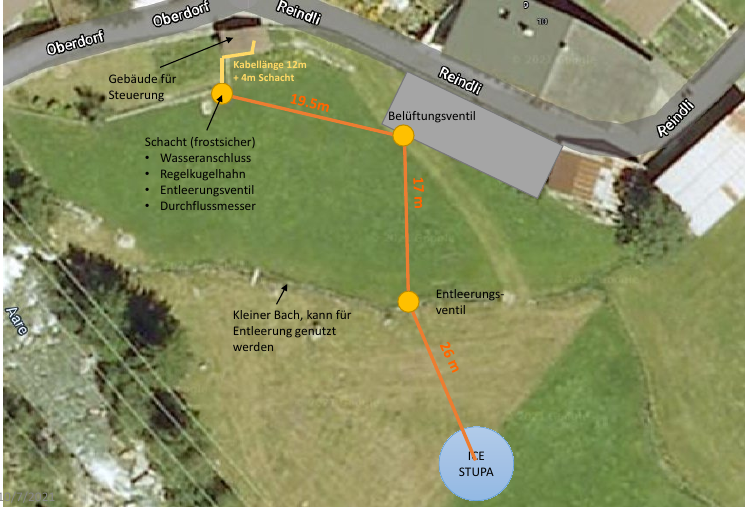
\includegraphics[width=\linewidth]{Figures/automation_system.png}
	\end{center}
  \caption{Guttannen automation system}
	\label{fig:layout}
\end{figure}

\subsubsection{Software}

The objective of the automation software is to estimate the freezing rate in the (a) least data demanding and
(b) computationally intensive way possible. Objective (a) is achieved by introducing assumptions to the energy
balance model used in \cite{balasubramanianInfluenceMeteorologicalConditions2022}. Objective (b) is achieved by formulating a surrogate empirical
model that best approximates the simplified physical model. 

% \subsubsection{Simplified physical model}

The growth rate of the AIR can be represented as: 

\begin{equation}
  \frac{\Delta V_{ice}}{\Delta t}  =  \frac{\Delta j_{cone}}{ \Delta t} \cdot A_{cone}
	\label{eqn:freeze}
\end{equation}

where $\frac{\Delta j_{cone}}{\Delta t}$ is the thickness change rate of the AIR which can be represented as: 

\begin{equation}
  \frac{\Delta j_{cone}}{\Delta t}  = \frac{1}{\rho_w} \cdot (\frac{q_{SW} + q_{LW} + q_{S} + q_{F} + q_{G}}{L_F} + \frac{q_{L}}{L_V} )
	\label{eqn:freeze}
\end{equation}

We reduce the data requirements for estimation of each of the energy flux components using assumptions that
underestimate the associated freezing rate in order to optimise for water use efficiency. Further description of
our assumptions are described in the Appendix. Below, we summarise the list of assumptions used:

\begin{itemize}

  \item Shortwave Radiation $q_{SW}$: The direct and diffuse components of shortwave radiation are estimated from the coordinates,
    altitude and time using the PVLIB python package described in \cite{holmgrenPvlibPythonPython2018} . The
    algorithm used to estimate the clear-sky global radiation is described in
    \cite{ineichenBroadbandSimplifiedVersion2008} and the algorithm used to estimate the diffuse part of the
    global radiation is described in \cite{erbsEstimationDiffuseRadiation1982}. The uncertainty of this approach
    is discussed in \cite{ineichenValidationModelsThat2016}. Furthermore, the solar area fraction is also
    approximated by assuming $h_{cone} = r_{cone} = r_{F}$ and the albedo is assumed to be equal to ice albedo
    (0.25). These assumptions underestimate the freezing rate.

  \item Longwave Radiation $q_{LW}$: We assume $T_{ice} = 0 \degree C$. This assumption overestimates $q_{LW}$
    and thereby underestimates the freezing rate.

  \item Turbulent fluxes ($q_{L}$ and $q_{S}$): The software estimates the pressure using the altitude of the
    location and ignores the $\mu_{cone}$ parameter thereby underestimating the turbulent fluxes.

  \item $q_{F}$ and $q_{G}$: We ignore the influence of fountain water heat flux and the ground heat flux
    thereby removing the need for water temperature measurements.

  \item Surface Area $A_{cone}$ : The area of the conical AIR is approximated to the area of its circular base
    produced through the fountain spray radius $r_F$. This assumption is derived from
    \cite{oerlemansBriefCommunicationGrowth2021} model and underestimates the surface area of the AIR during the
    accumulation period and thereby underestimates the freezing rate.

\end{itemize}

% \subsubsection{Surrogate empirical model}

We can now construct a surrogate model that approximates the thickness change rate into a computationally
inexpensive equation with fixed coefficients. We approximate the shortwave radiation flux using a gaussian
function $g($ hour of day $)$ that accounts for its diurnal variation. The gaussian equation's three
coefficients are calibrated based on estimation of solar radiation during the last day of the construction
period. We approximate the rest of the energy fluxes by assuming a linear relationship with the weather
parameters namely, temperature, humidity, wind speed and altitude. Using the above simplifications, we can
compute the expected thickness change rates using the following set of equations:

% \begin{subequations}
% 	\begin{align}
% 		\label{eqn:sun}
%   \frac{q_{SW}}{\rho_w \cdot L_F} & \approx \frac{amp}{(\sigma \sqrt{2\pi})} \cdot
%   exp\left(\frac{-(hod-\mu)^2}{2\sigma^2}\right) = g(hod)  \\
% 		\label{eqn:T}
%    \frac{q_{LW} + q_{S}}{\rho_w \cdot L_F} + \frac{q_L}{\rho_w \cdot L_V} & \approx a \cdot T_a + b \cdot RH + c \cdot v_a +
%   d \cdot alt + e = f(T_a, RH, v_a, alt) \\
% 		\label{eqn:auto}
%   \frac{\Delta j_{cone}}{\Delta t} & \approx g(hod) + f(T_a, RH, v_a, alt)
% 	\end{align}
% \end{subequations}

% where $r_F$ is the fountain spray radius and $hod$ is the hour of day.


% \begin{table}[ht]
% \centering
% \caption{}
% \label{tab:my-table}
% \begin{tabular}{@{}lllllll@{}}
% \toprule
% Coefficients of & $T_a\, [\degree C]$ & $RH\,[\%]$ & $v_a\, [m\, s^{-1}]$ & $alt\, [km]$  & $constant$ \\ \midrule
% Value           & $\num{-5.6 e-3}$     & $\num{-3.2 e-4}$ & $\num{4.7 e-3}$ & $\num{-3.5 e-3}$  & $\num{5.2 e-3}$
%                 \\ \bottomrule
% \end{tabular}
% \end{table}


\subsubsection{User interface}
The software is configured in such a way that it works independently of a PC. Once switched on, the software
starts automatically. The system runs if none of the following termination criteria apply:

\begin{itemize}
\item Wind speed greater than limit value
\item Ambient temperature higher or lower than limit values
\item Pipeline freezing event detected: $IW_{KH} > 20 \%$ and $Q_w = 0$ for atleast 20 seconds (Icing)
\item Leakage detected: $Q_w > 65 l/min$
\end{itemize}

\begin{figure}[ht]
	\begin{center}
		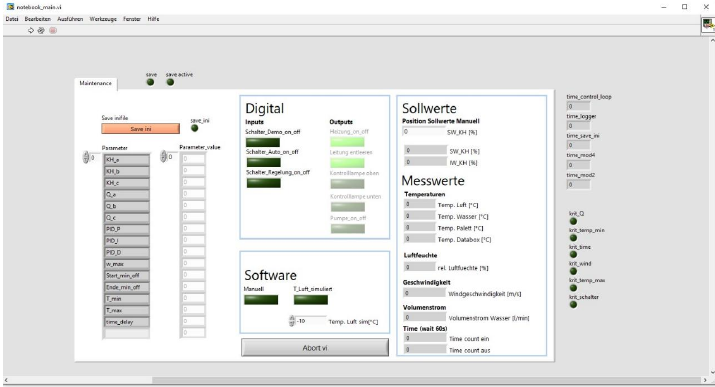
\includegraphics[width=\linewidth]{Figures/user_interface.png}
	\end{center}
  \caption{User Interface}
	\label{fig:UI}
\end{figure}



\section{Results}
\subsection{Model comparison}
Nash equation

\subsubsection{Shortwave radiation comparison}

\subsubsection{Freezing rate comparison}

\subsection{Ice Volume Validation}

\begin{figure}[ht]
	\begin{center}
		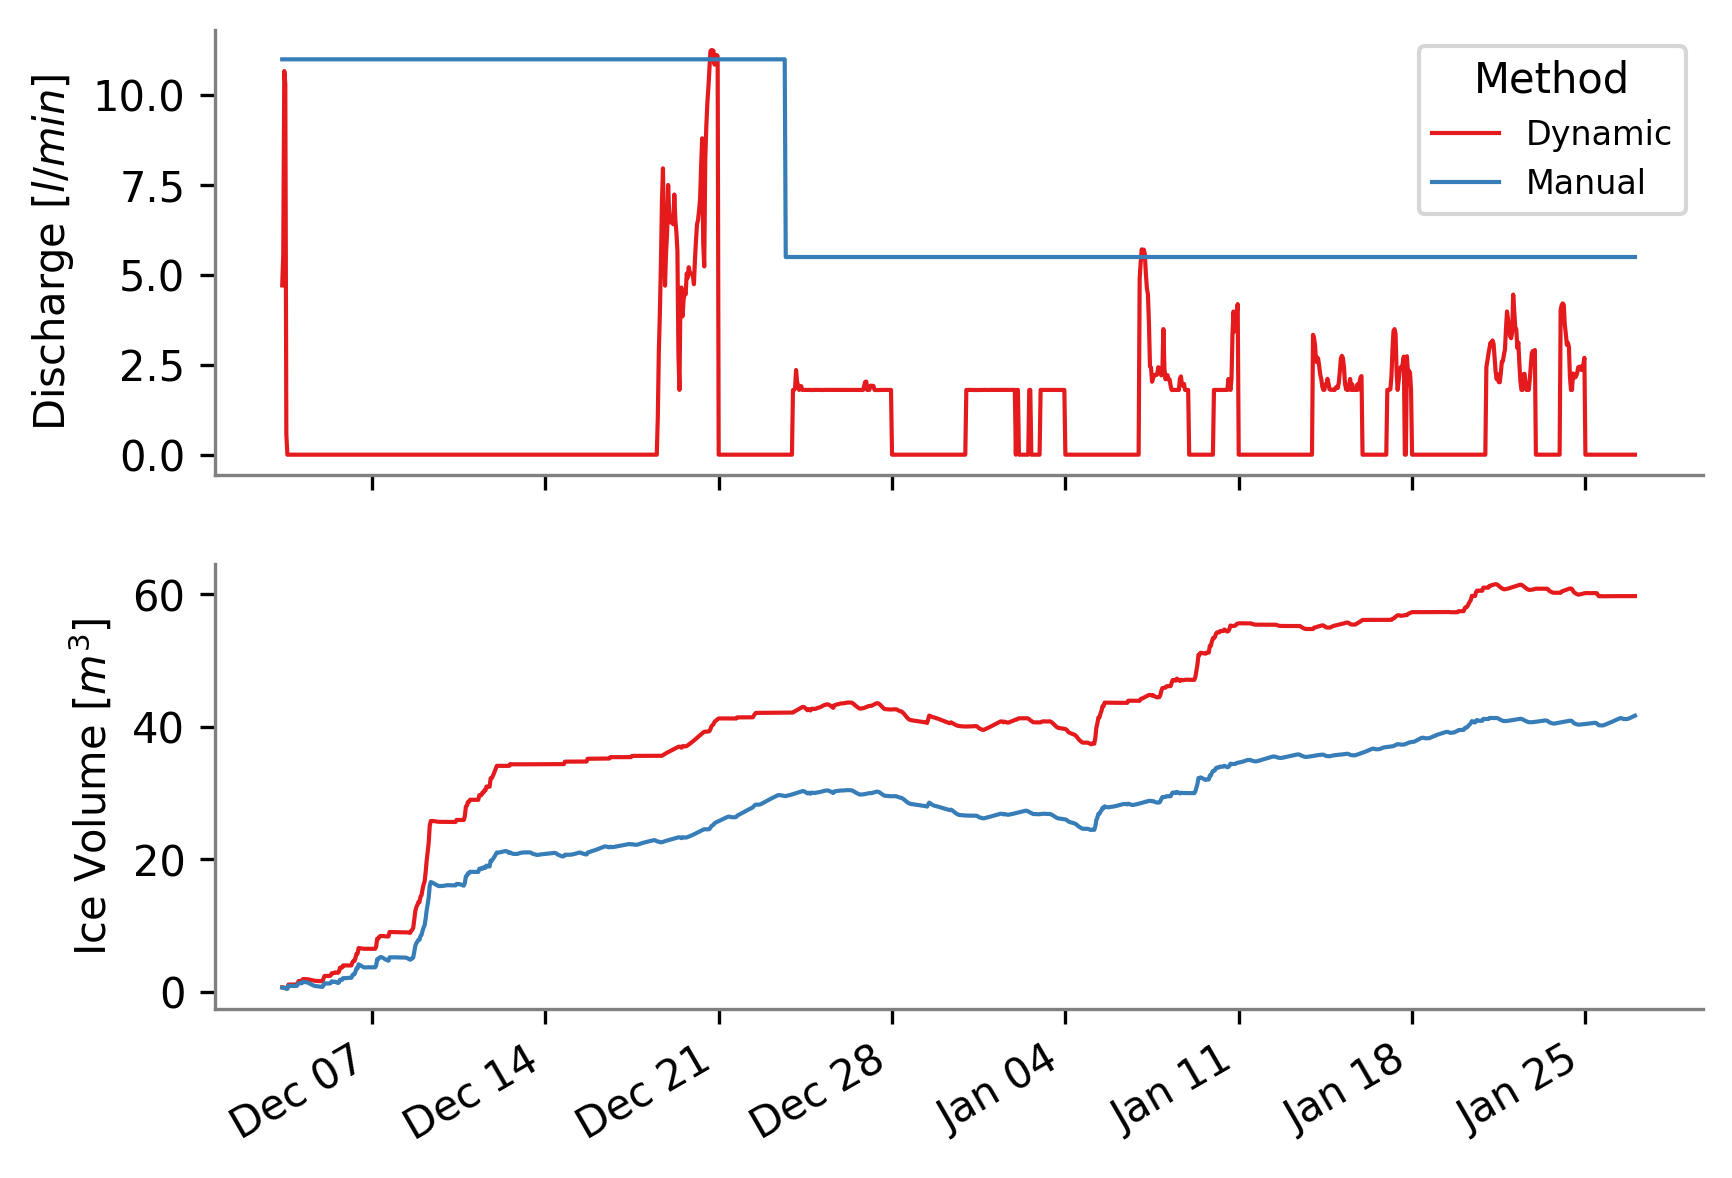
\includegraphics[width=\linewidth]{Figures/autovsman_dis.png}
	\end{center}
	\caption{Comparison of discharge and ice volume between AIRs produced by dynamic and static fountains. }
	\label{fig:old_icestupa}
\end{figure}



% \begin{figure}[ht]
% 	\begin{center}
% 		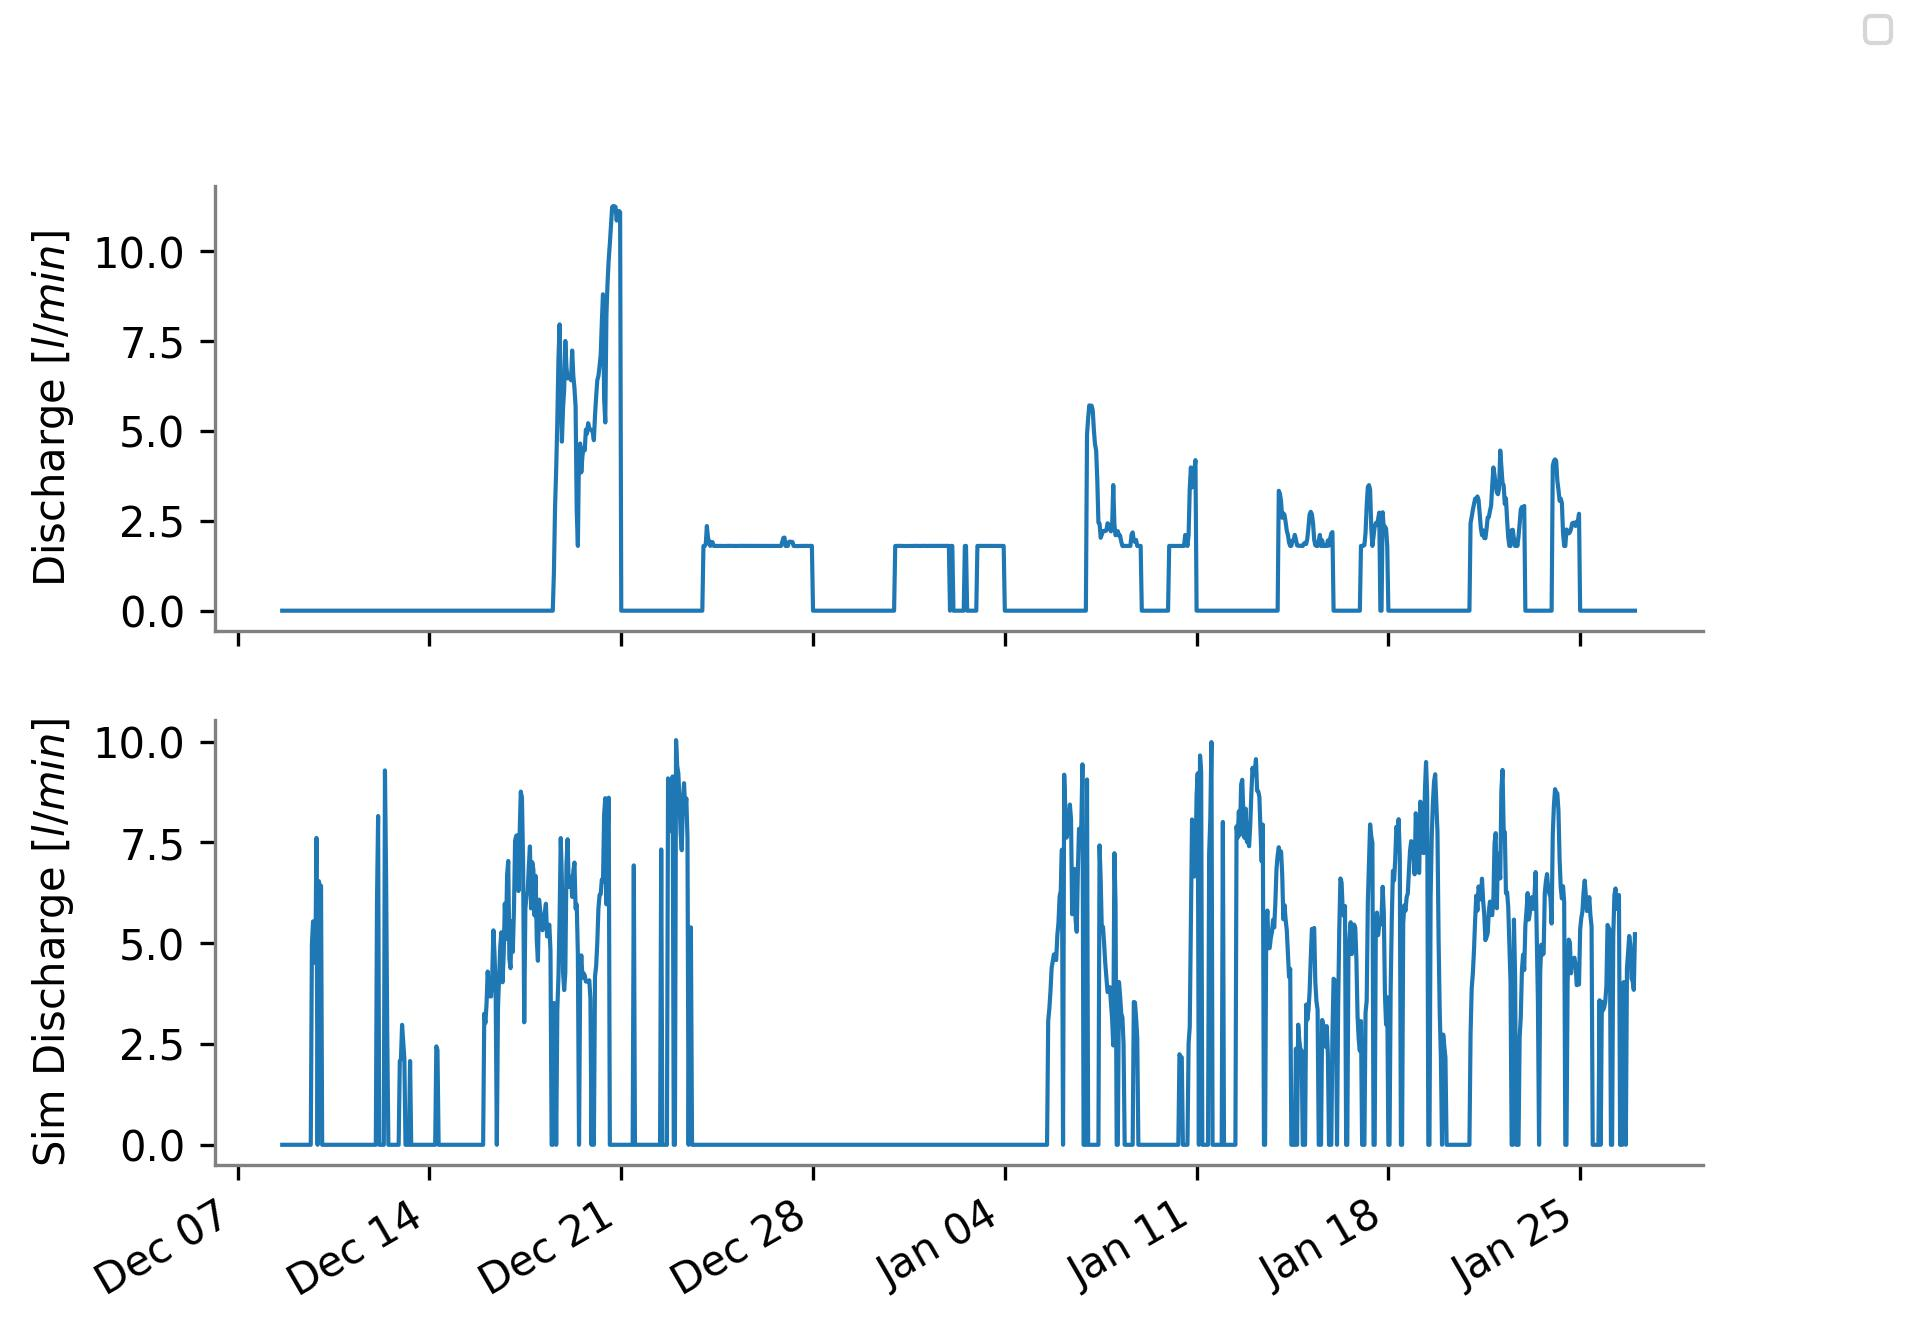
\includegraphics[width=\linewidth]{Figures/simvsreal_dis.jpg}
% 	\end{center}
% 	\caption{Comparison of discharge and ice volume between AIRs produced by dynamic and static fountains. }
% 	\label{fig:old_icestupa}
% \end{figure}



\subsection{Water Use efficiency}

\begin{figure}[ht]
	\begin{center}
		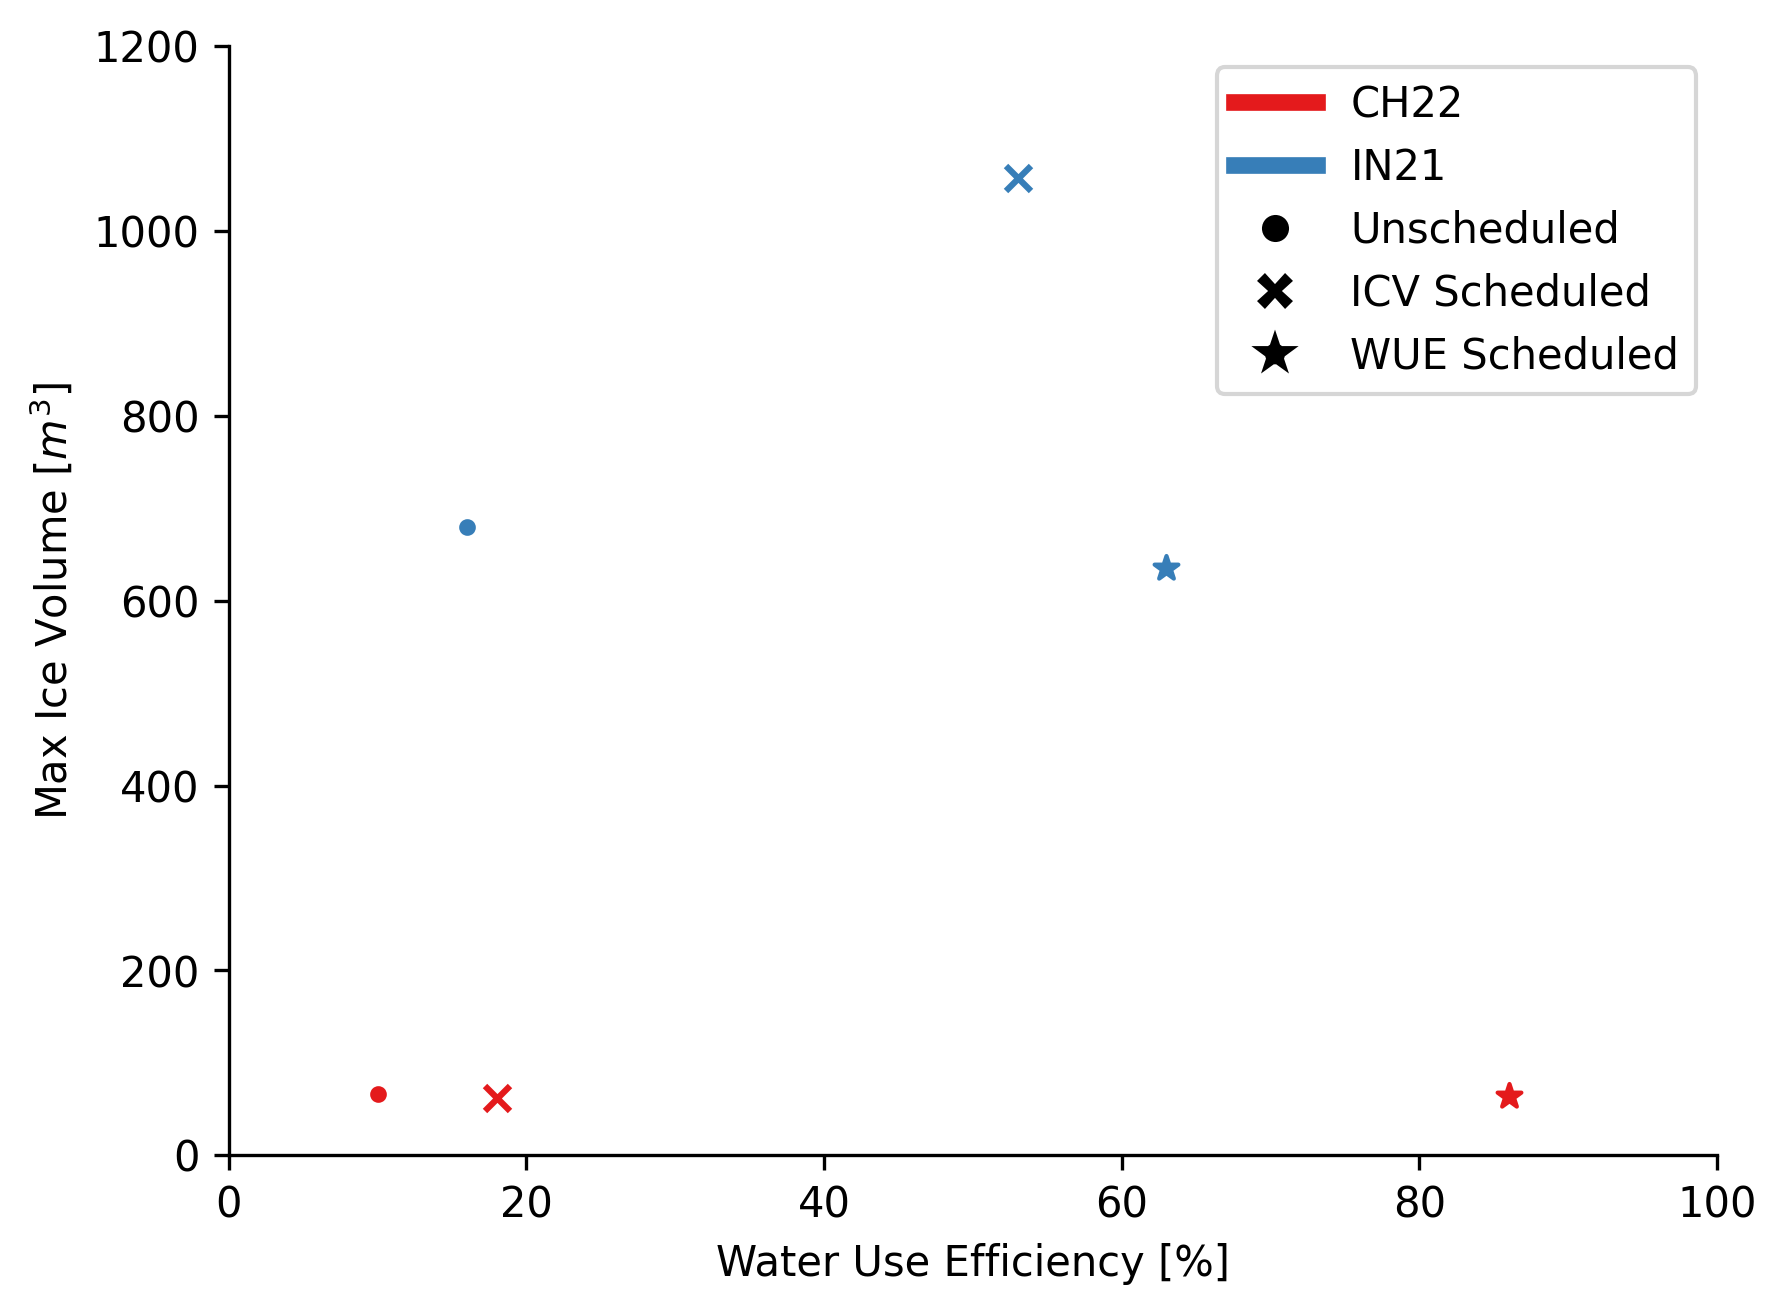
\includegraphics[width=\linewidth]{Figures/wue.png}
	\end{center}
	\caption{Comparison of discharge and ice volume between AIRs produced by dynamic and static fountains. }
	\label{fig:old_icestupa}
\end{figure}

\section{Discussion}
\subsection{Limited and unlimited water availability}

\subsection{Fountain vs weather influence}

\subsection{Ideal fountains and locations for AIR construction}

\subsection{Fountain height and spray radius}

\subsection{Eddy covariance comparison}

\subsection{Surface temperature}

\subsection{Implementation costs}

Since this technology is currently being used by subsistence farmers, we also need to be mindful of the
maintenance and implementation costs. We propose two different modes of fountain scheduling based on operation
costs that can be classified as static or dynamic. In the static mode, the total amount of water
for AIR construction is allocated without specifying its temporal distribution along the accumulation period. By
contrast, in the dynamic mode water is allocated at specific time steps along the accumulation period in
order to achieve even higher WUE.

Both the approaches use a fountain and pipeline system with minimal manual intervention. The dynamic mode is
better suited for locations where the diurnal and seasonal variations in the weather conditions are significant.
In such cases, the real-time adjustments of the discharge rate make efficient fountain scheduling
possible. The static mode is better suited for other locations or for users who cannot afford the additional
hardware requirements to implement the dynamic fountain scheduling mode.

\section{Conclusions}


In this paper, two different construction strategies that yield better water use efficiency are presented.
An automation system was developed to implement the dynamic fountain sischarge mode and tested using data
collected at Guttannen, Switzerland during the 2021-22 winter season. 

The main purpose of this study was to test the idea that scheduling AIR fountain systems could lead to a
significant improvement in water use efficiency.

This study has demonstrated the importance of fountain scheduling. Furthermore, the decrease in performance of
the empirical model has been quantified through comparison of efficiency criteria. The study has demonstrated
that, it is possible to compute more than 90 \% of the freeze rate variations by means of a simplified empirical
model. This model satisfies the need for a less data demanding and computationally intensive workflow for
scheduling fountains worldwide using the computation of just 6 coefficents. Such a model will be compatible with
the limited data amount that is typical of any new AIR construction location.

This study has also compared the sensitivity of freezing rates between the weather components and the fountain's
spray radius. It is clear that if improvements are to be achieved, future research must be devoted to modelling
the impact of fountain design on the spray radius.

The model discussed in this paper will be applied worldwide to identify favourable AIR locations in a future
paper.


The automation system allows the easy handling of fountain scheduling implementation. Its capabilities for
achieving a higher water saving was tested for Guttannen. The possibility for easily changing the automation
coefficients allows tailoring the fountain discharge rate according to identified requirements. Other on-going
improvements concern the use of the automation software as a decision support tool applicable at both the local
and the global scale.

\section{Appendix}

The area of the conical AIR is approximated to the area of its circular base produced through the fountain spray
radius $r_F$. Therefore, the surface area can be determined using

\begin{equation} A_{cone} =\pi \cdot r_{F}^2 \label{eq:Area} \end{equation}

Admittedly, this assumption underestimates the surface area of the AIR during the accumulation period and
thereby underestimates the freezing rate.

We approximate the energy balance at the surface of an AIR by a one-dimensional description of energy fluxes as
used in \cite{balasubramanianInfluenceMeteorologicalConditions2022}:


Upward and downward fluxes relative to the ice surface are positive and negative, respectively. The first term
represents the energy change used for freezing the fountain water and melting the ice. $q_{SW}$ is the net
shortwave radiation; $q_{LW}$ is the net longwave radiation; $q_{L}$ and $q_{S}$ are the turbulent latent and
sensible heat fluxes. 

The software assumes $T_{ice} = 0 \degree C$ and therefore ignores the temperature change flux $q_{T}$, fountain
heat flux $q_{F}$ and ground heat flux $q_{G}$. All these assumptions overestimate the freezing rate.

Furthermore, we the rest of the energy balance components based on their air temperature and solar
radiation dependence. Namely, $q_{LW}$, $q_{L}$ and $q_{S}$ contribute to temperature induced freeze rate and
$q_{SW}$ contributes to solar radiation induced melt rate during the accumulation period.  Particularly,

For the static method, we only need to determine the night freezing rates whereas for the dynamic approach we
also need to account for the day melt during the accumulation period.

\subsection{Net Longwave radiation \texorpdfstring{$q_{LW}$}{Lg}} \label{sec:LW}
The net longwave radiation $q_{LW}$ is determined as follows:

\begin{equation}
	q_{LW}= \sigma \cdot \epsilon_a \cdot {(T_a+ 273.15)}^4 -\sigma \cdot \epsilon_{ice} \cdot {(T_{ice}+ 273.15)}^4
	\label{eqn:LW}
\end{equation}

where $T_a$ represents the measured air temperature, $\epsilon_a$ denotes the atmospheric emissivity $T_{ice}$
is the modelled surface temperature given in [$\degree C$], $\sigma=5.67\cdot10^{-8}\,Jm^{-2}s^{-1}K^{-4}$ is
the Stefan-Boltzmann constant and $\epsilon_{ice}$ is the corresponding emissivity value for the Icestupa
surface (0.97).

We approximate the atmospheric emissivity $\epsilon_a$ ,
considering air temperature and vapor pressure (Eqn. \ref{eqn:atm_e}). The vapor pressure of air over water and
ice was obtained using Eqn. \ref{eqn:vp}.  The expression defined in \cite{brutsaertDerivableFormulaLongwave1975} for clear skies
(first term in equation \ref{eqn:atm_e}) is extended with the correction for cloudy skies after
\cite{brutsaertEvaporationAtmosphereTheory1982} as follows:

\begin{equation}
	\epsilon_a=1.24 \cdot (\frac{p_{v,w}}{(T_a+273.15)})^{1/7}\cdot(1+0.22\cdot{cld}^2) \label{eqn:atm_e}
\end{equation}

with a cloudiness index $cld$, ranging from 0 for clear skies to 1 for complete overcast skies. 

The software assumes $T_{ice} = 0 \degree C$. This assumption overestimates $q_{LW}$ and thereby underestimates
the freezing rate.

\subsection{Turbulent fluxes} \label{sec:Qs}

The turbulent sensible $q_{S}$ and latent heat $q_{L}$ fluxes are computed with the following expressions
proposed by \cite{garrattAtmosphericBoundaryLayer1992}:

\begin{equation}
	q_{S}= c_{a} \cdot \rho_{a} \cdot p_{a}/p_{0,a} \cdot \frac{\kappa^2 \cdot v_a \cdot
		(T_a-T_{ice})}{{(\ln{\frac{h_{AWS}}{z_{0}}})}^2}
	\label{eqn:qs}
\end{equation}

\begin{equation}
	q_{L}= 0.623 \cdot L_s \cdot \rho_{a}/p_{0,a} \cdot \frac{\kappa^2 \cdot
	v_a(p_{v,w}-p_{v,ice})}{{(\ln{\frac{h_{AWS}}{z_{0}}})}^2}
\end{equation}

where $h_{AWS}$ is the measurement height above the ground surface of the AWS (around $2\,m$ for all sites),
$v_a$ is the wind speed in [$m\,s^{-1}$], $c_a$ is the specific heat of air at constant pressure (1010 J
$kg^{-1} K^{-1}$), $\rho_{a}$ is the air density at standard sea level (1.29 $kg m^{-3}$), $p_{0,a}$ is the air
pressure at standard sea level (1013 $hPa$), $p_{a}$ is the measured air pressure, $\kappa$ is the von Karman
constant (0.4), $z_{0}$ is the surface roughness (3 $mm$) and $L_s$ is the heat of sublimation (2848
$kJ\,kg^{-1}$).  The vapor pressure of air with respect to water ($p_{v,w}$) and with respect to ice
($p_{v,ice}$) was obtained using the formulation given in \cite{huangSimpleAccurateFormula2018} :

\begin{equation}
	\begin{split}
		p_{v,w}&=e^{\frac{(34.494 - \frac{4924.99}{T_{a} + 237.1})}{(T_a + 105)^{1.57} \cdot 100}} \cdot \frac{RH}{100} \\
		p_{v,ice}&=e^{\frac{(43.494 - \frac{6545.89}{T_{ice} + 278})}{(T_{ice} + 868)^{2} \cdot 100}} \\
	\end{split} \label{eqn:vp}
\end{equation}

The software ignores the $\mu_{cone}$ parameter thereby underestimating the turbulent fluxes. Since turbulent
fluxes impact both the freezing and the melting rates, this assumption may not underestimate freezing rates.

\subsection{Net shortwave radiation \texorpdfstring{$q_{SW}$}{Lg}}
\label{sec:SW}

The net shortwave radiation $q_{SW}$ is computed as follows:

\begin{equation} q_{SW} = (1- \alpha_{ice}) \cdot ( SW_{direct} \cdot f_{cone} + SW_{diffuse})
\label{eqn:SW} \end{equation}

where $\alpha_{ice}$ is the bare ice albedo value (0.25); $SW_{direct}$ is the direct shortwave radiation. The
global shortwave radiation used is modelled using the parametrisation proposed by \cite{woolfComputationSolarElevation1968}.

The solar area fraction $f_{cone}$ of the ice structure exposed to the direct shortwave radiation depends on the
shape considered. Using the solar elevation angle $\theta_{sun}$, the solar beam can be considered to have a
vertical component, impinging on the horizontal surface (semicircular base of the AIR), and a horizontal
component impinging on the vertical cross section (a triangle). The solar elevation angle $\theta_{sun}$ used is
modelled using the parametrisation proposed by \cite{woolfComputationSolarElevation1968}. Here we overestimate the impact of direct
solar radiation by assuming $h_{cone} = r_{cone} = r_{F}$. Accordingly, $f_{cone}$ is determined as follows:

\begin{equation}
	\begin{split}
		f_{cone}& =\frac{ cos \theta_{sun} + \pi \cdot sin \theta_{sun} }{2\sqrt{2} \cdot \pi }\\
	\end{split}
	\label{ eqn:f_{cone}}
\end{equation}

The software ignores the variations in the albedo and assumes it to be equal to that of ice to simplify the
model. This assumption overestimates the solar radiation absorption thereby underestimating the freezing rate.


\bibliographystyle{frontiersinSCNS_ENG_HUMS} \bibliography{zot_refs}

\end{document}

% \begin{landscape}
% \begin{table}[]
% \centering
% \caption{}
% \label{tab:my-table}
% \begin{tabular}{@{}lllll@{}}
% \toprule
% \textbf{Module name} & \textbf{Symbol} & \textbf{Full eqn} & \textbf{Simplified eqn} & \textbf{Assumptions} \\ \midrule
% \multicolumn{1}{|l}{Surface Area}        & $A_{cone}$ &  & \pi \cdot r_{F}^2 & \multicolumn{1}{l|}{} \\ \midrule
% \multicolumn{1}{|l}{Shortwave Radiation} & $q_{SW}$ &  & (1- \alpha_{ice}) \cdot ( (1- cld) \cdot SW_{global} \cdot f_{cone} + cld \cdot SW_{global}) & \multicolumn{1}{l|}{} \\ \midrule
% \multicolumn{1}{|l}{Longwave Radiation}  & $q_{LW}$ &  & \sigma \cdot \epsilon_a \cdot {(T_a+ 273.15)}^4 -\sigma \cdot \epsilon_{ice} \cdot {273.15}^4 & \multicolumn{1}{l|}{} \\ \midrule
% \multicolumn{1}{|l}{Sensible Heat}       & $q_{S}$ &  &  & \multicolumn{1}{l|}{} \\ \midrule
% \multicolumn{1}{|l}{Latent Heat}         & $q_{L}$ &  &  & \multicolumn{1}{l|}{} \\ \bottomrule
% \multicolumn{1}{|l}{Temperature heat flux} & $q_{T}$ &  & 0 & \multicolumn{1}{l|}{} \\ \bottomrule
% \multicolumn{1}{|l}{Fountain discharge heat flux} & $q_{F}$ &  & 0 & \multicolumn{1}{l|}{} \\ \bottomrule
% \multicolumn{1}{|l}{Ground heat flux}    & $q_{G}$ &  & 0 & \multicolumn{1}{l|}{} \\ \bottomrule
% \end{tabular}
% \end{table}
% \end{landscape}
